% !TeX root = thesis.tex

\chapter{Related work}
In the previous chapter I have stressed the paramount importance of periodically integrating one's changes into the upstream repository. Additionally, Continuous Integration was introduced as both a practice and a tool to facilitate this often complex and time-consuming process. However, Continuous Integration is not the golden bullet for software engineering. In this chapter I will investigate the flip side of applying this practice. After every integration, all of the unit and regression tests in the test suite must be executed to ensure that the integration was successful and that no new bugs have been introduced. As the project evolves, the size of the codebase increases and consequently the amount of tests will increase as well in order to maintain a sufficiently high coverage level. An increase in the size of the test suite will inevitably lead to an increase in test duration \cite{evaluationoftestsuiteminimization}, which imposes an issue of scaling. Walcott, Soffa and Kapfhammer illustrate the magnitude of this problem by providing an example of a codebase consisting of 20.000 lines, for which the tests require up to seven weeks to complete \cite{10.1145/1146238.1146240}.\\

\noindent Fortunately, multiple developers and researchers have found some techniques that can help to resolve this issue. I will describe the existing methods in the below section and afterwards I will conclude this chapter by providing an overview of existing implementations in software of the discussed techniques.

\section{Classification of approaches}
In literature, three distinct approaches are currently known to handle the scalability issues of growing test suites. Developers can either apply \emph{\tsm{}}, \emph{\tcs{}} or \emph{\tcp{}} \cite{evaluationoftestsuiteminimization}. All three algorithms can be applied to any set of tests, however there is a trade-off to be made. Depending on which algorithm is chosen, it will have a major impact on the duration of the test suite duration in exchange for a reduced test coverage level. I will now elaborate on the details of these three approaches.

% !TeX root = ../../thesis.tex

\subsection{\tsm{}}
\label{ssec:tsm}
The first technique is called \acrfull{tsm}, also referred to as \emph{Test Suite Reduction} in literature. This technique will try to reduce the size of the test suite by permanently removing redundant test cases. This problem has been formally defined by Rothermel \cite{10.1002/stv.430} in \cref{def:tsm} and illustrated in \Cref{fig:tsm}.

\begin{definition}[\tsm{}]
\label{def:tsm}
\mbox{}\\Given:
\begin{itemize}
	\item $T = \{t_1, \dots, t_n\}$ a test suite consisting of test cases $t_j$.
	\item $R = \{r_1, \dots, r_m\}$ a set of requirements that must be satisfied in order to provide the desired ``adequate'' testing of the program.
	\item $\{T_1, \dots, T_m\}$ subsets of test cases in $T$, such that for every $i \in [1..m]$, any one of the test cases $t_j \in T_i$ can be used to satisfy requirement $r_i$.
\end{itemize}

\noindent Subsequently, we can define \tsm{} as the task of finding a subset $T'$ of test cases $t_j \in T$ that satisfies every requirement $r_i$.
\end{definition}

\noindent If we apply the concepts of the previous chapter to the above definition, we can interpret the set of requirements $R$ as source code lines that must be covered. A requirement $r_i$ can subsequently be satisfied by any test case $t_j \in T$ that belongs to the subset $T_i$. Observe that the problem of finding $T'$ is closely related to the \emph{hitting set problem} (\cref{def:hitting-set}) \cite{10.1002/stv.430}.

\begin{definition}[Hitting Set Problem]
\label{def:hitting-set}
\mbox{}\\Given:
\begin{itemize}
	\item $S = \{s_1, \dots, s_n\}$ a finite set of elements.
	\item $C = \{c_1, \dots, c_n\}$ a collection of sets, with $\forall c_i \in C : c_i \subseteq S$.
\end{itemize}

\noindent The hitting set is a subset $S' \subseteq S$ such that $S'$ contains at least one element from each subset in $C$.
\end{definition}

\noindent In the context of \tsm{}, $T'$ corresponds to the hitting set of $T_i$s. In order to effectively minimise the amount of tests in the test suite, $T'$ should be the minimal hitting set \cite{10.1002/stv.430}. Since we can reduce this problem to the NP-complete \emph{Vertex Cover}-problem, we know that this problem is NP-complete as well \cite{10.5555/574848}.

\begin{figure}[htbp!]
	\centering
	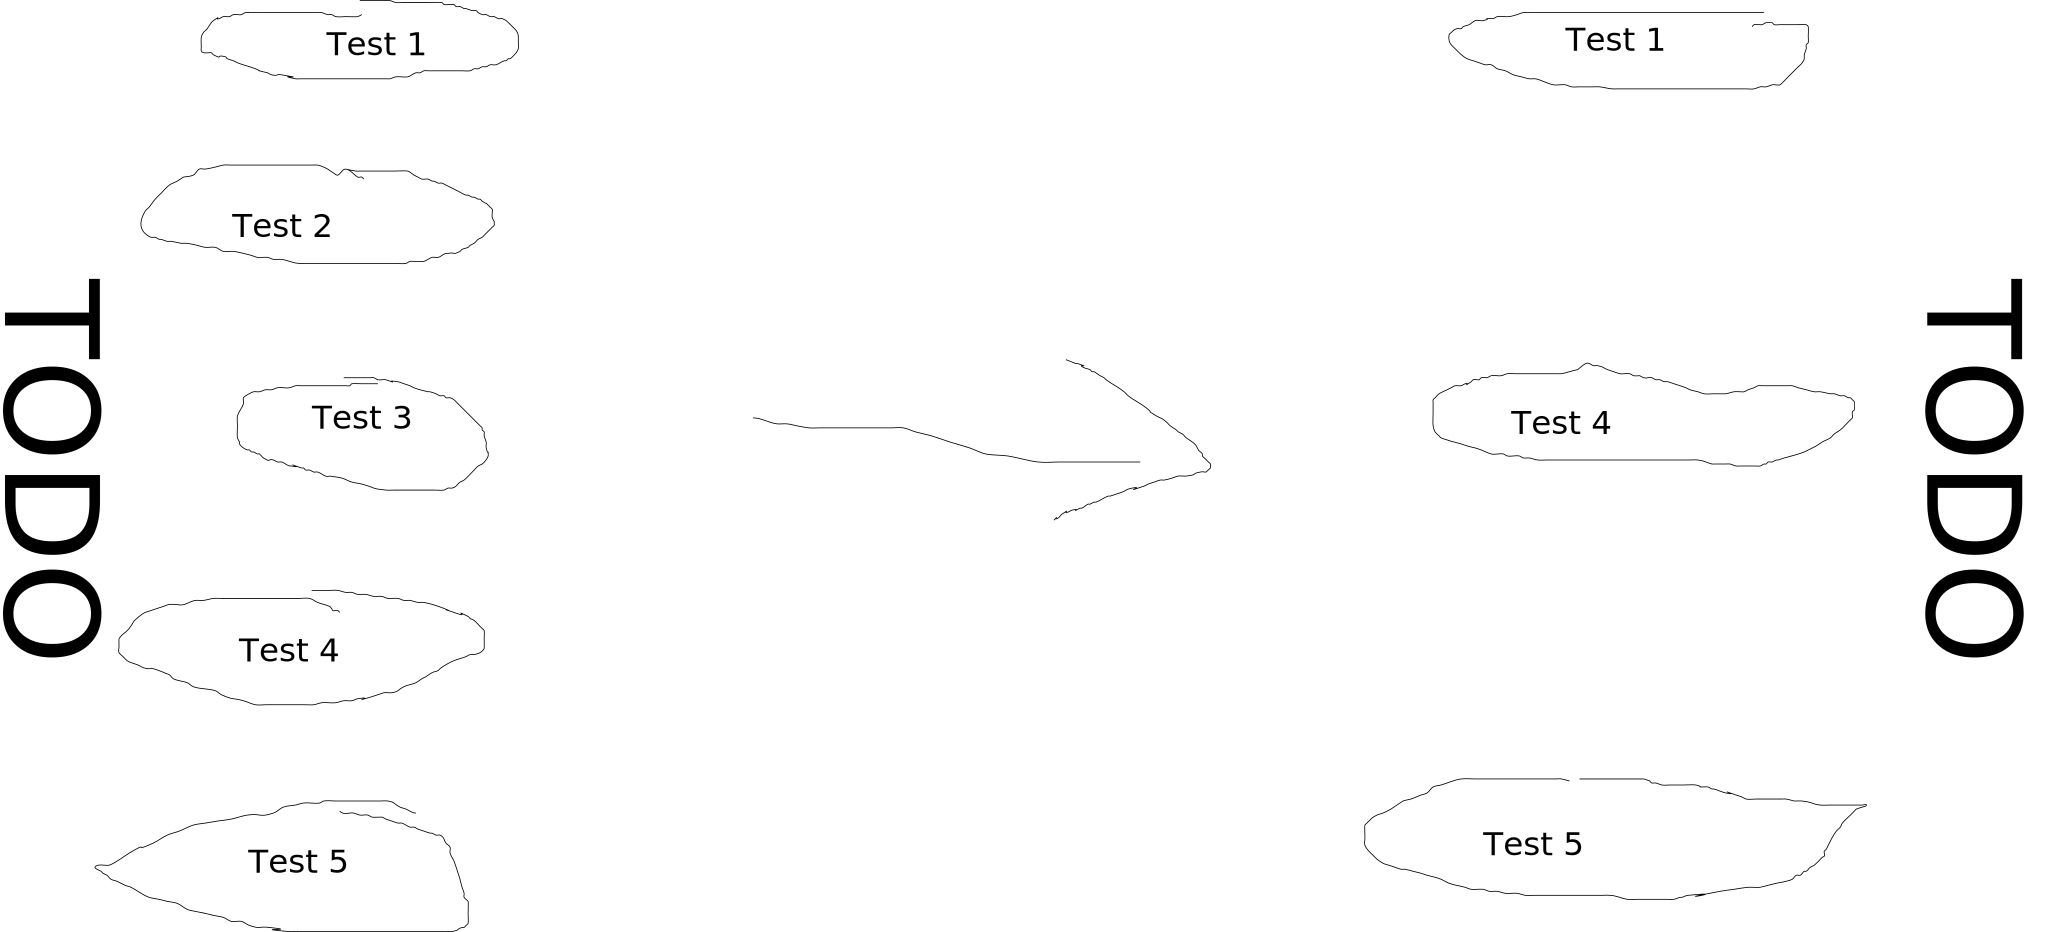
\includegraphics[width=\textwidth]{assets/tikz/approach-tsm.tikz}
	\caption{\tsm{}.}
	\label{fig:tsm}
\end{figure}
% !TeX root = ../../thesis.tex

\subsection{\tcs{}}
The second algorithm closely resembles the previous one. Instead of determining the minimal hitting set of the test suite in order to permanently remove tests, this algorithm has a notion of context. Prior to the execution of the tests, the algorithm performs a \emph{white-box static analysis} of the codebase to identify which parts have been changed. Subsequently, only the tests regarding modified parts are executed, making the selection temporary (\autoref{fig:tcs}) and modification-aware \cite{10.1002/stv.430}. Rothermel and Harrold define this formally in \autoref{def:tcs}.

\begin{definition}[\tcs{}]
\label{def:tcs}
\mbox{}\\Given:
\begin{itemize}
	\item $P$ the previous version of the codebase
	\item $P'$ the current (modified) version of the codebase
	\item $T$ the test suite
\end{itemize}

\noindent \tcs{} aims to find a subset $T' \subseteq T$ that is used to test $P'$. 
\end{definition}

\begin{figure}[htbp!]
	\centering
	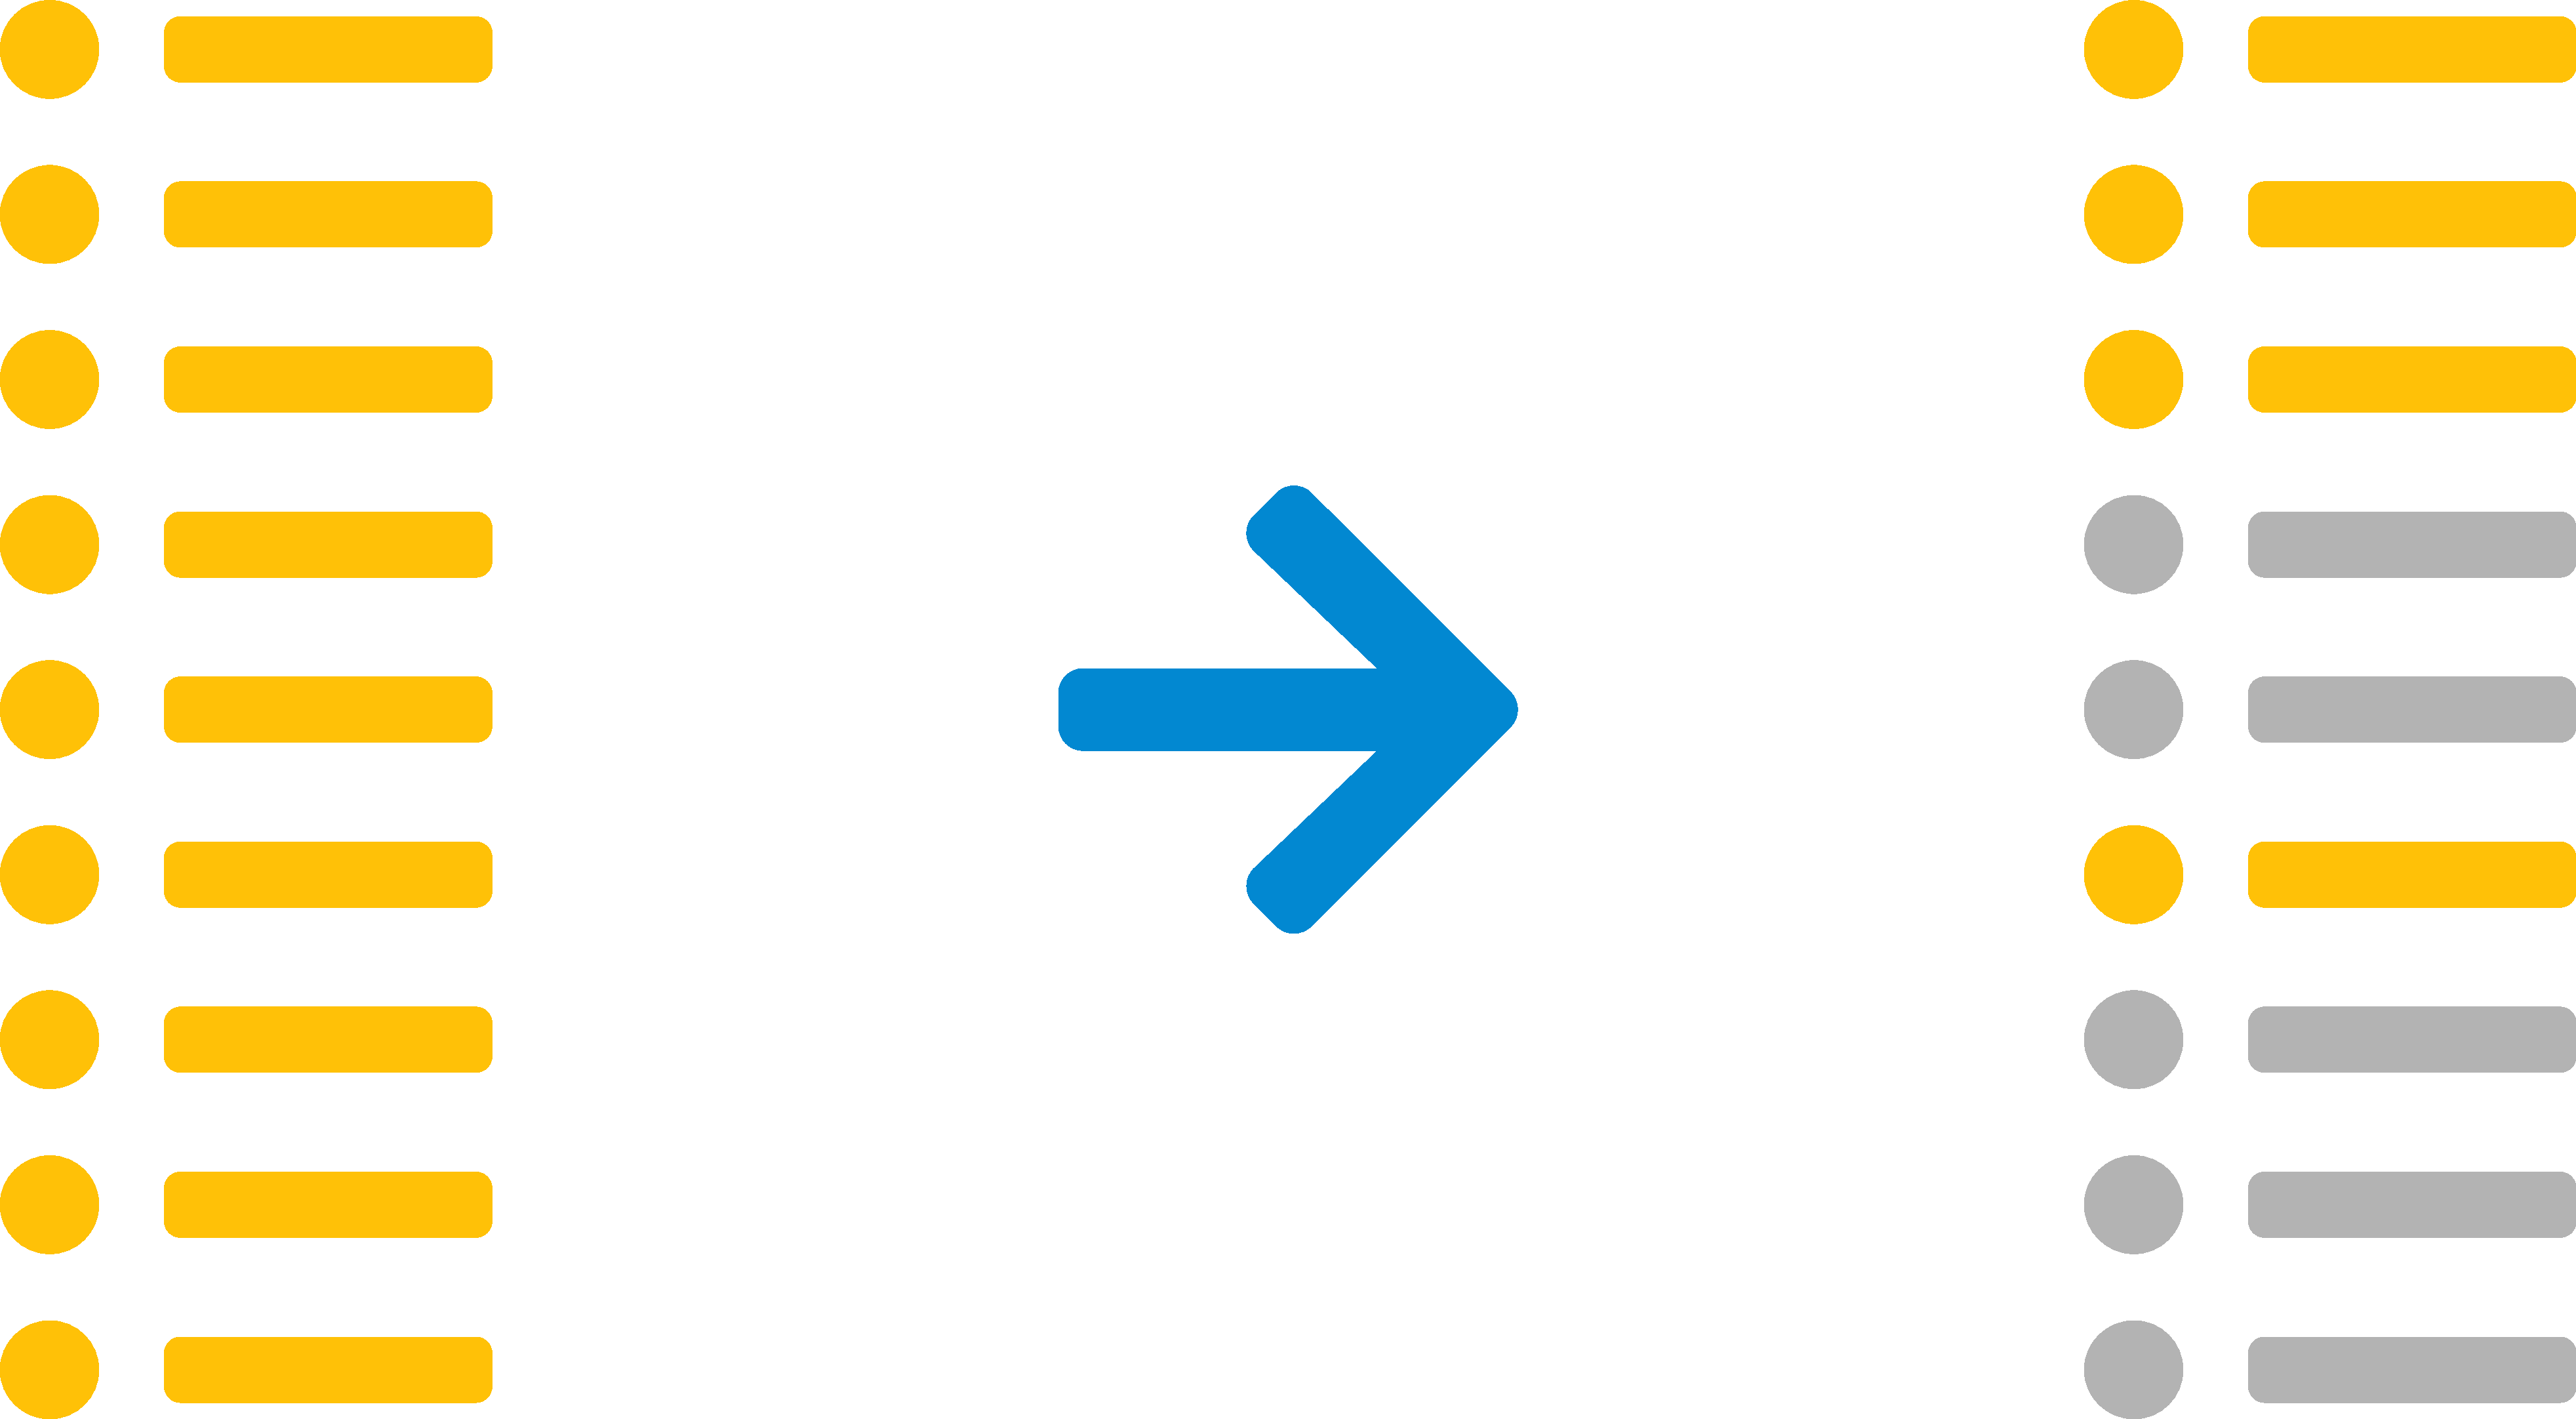
\includegraphics[width=0.8\textwidth]{assets/approach-tcs.pdf}
	\caption{\tcs{}}
	\label{fig:tcs}
\end{figure}
% !TeX root = ../../thesis.tex

\subsection{\tcp{}}
Both \acrshort{tsm} and \acrshort{tcs} attempt to execute as few tests as possible to reduce the execution time of the test suite. Nevertheless, in some cases, we may require to execute every test case to guarantee correctness. In this situation, we can still optimise the test suite. \acrfull{tcp} aims to find a permutation of the sequence of test cases, rather than eliminating specific tests from being executed (\Cref{fig:tcp}). We choose the order of the permutation in such a way that we can complete a predefined objective as soon as possible. Once we have achieved our objective, we can early terminate the execution of the test suite. In the worst-case scenario, we will still execute every test case. Some examples of objectives include covering as many lines of code as fast as possible or executing tests ordered on their probability of failure \cite{10.1002/stv.430}. \Cref{def:tcp} provides a formal definition of this approach.

\begin{definition}[\tcp{}]
\label{def:tcp}
\mbox{}\\Given:
\begin{itemize}
	\item $T$ the test suite
	\item $PT$ the set of permutations of $T$
	\item $f: PT \mapsto \mathbb{R}$ a function from a subset to a real number, this function is used to compare sequences of test cases to find the optimal permutation.
\end{itemize}

\noindent \tcp{} finds a permutation $T' \in PT$ such that $\forall T'' \in PT : f(T') \ge f(T'') \Rightarrow (T'' \ne T')$ 
\end{definition}

\begin{figure}[htbp!]
	\centering
	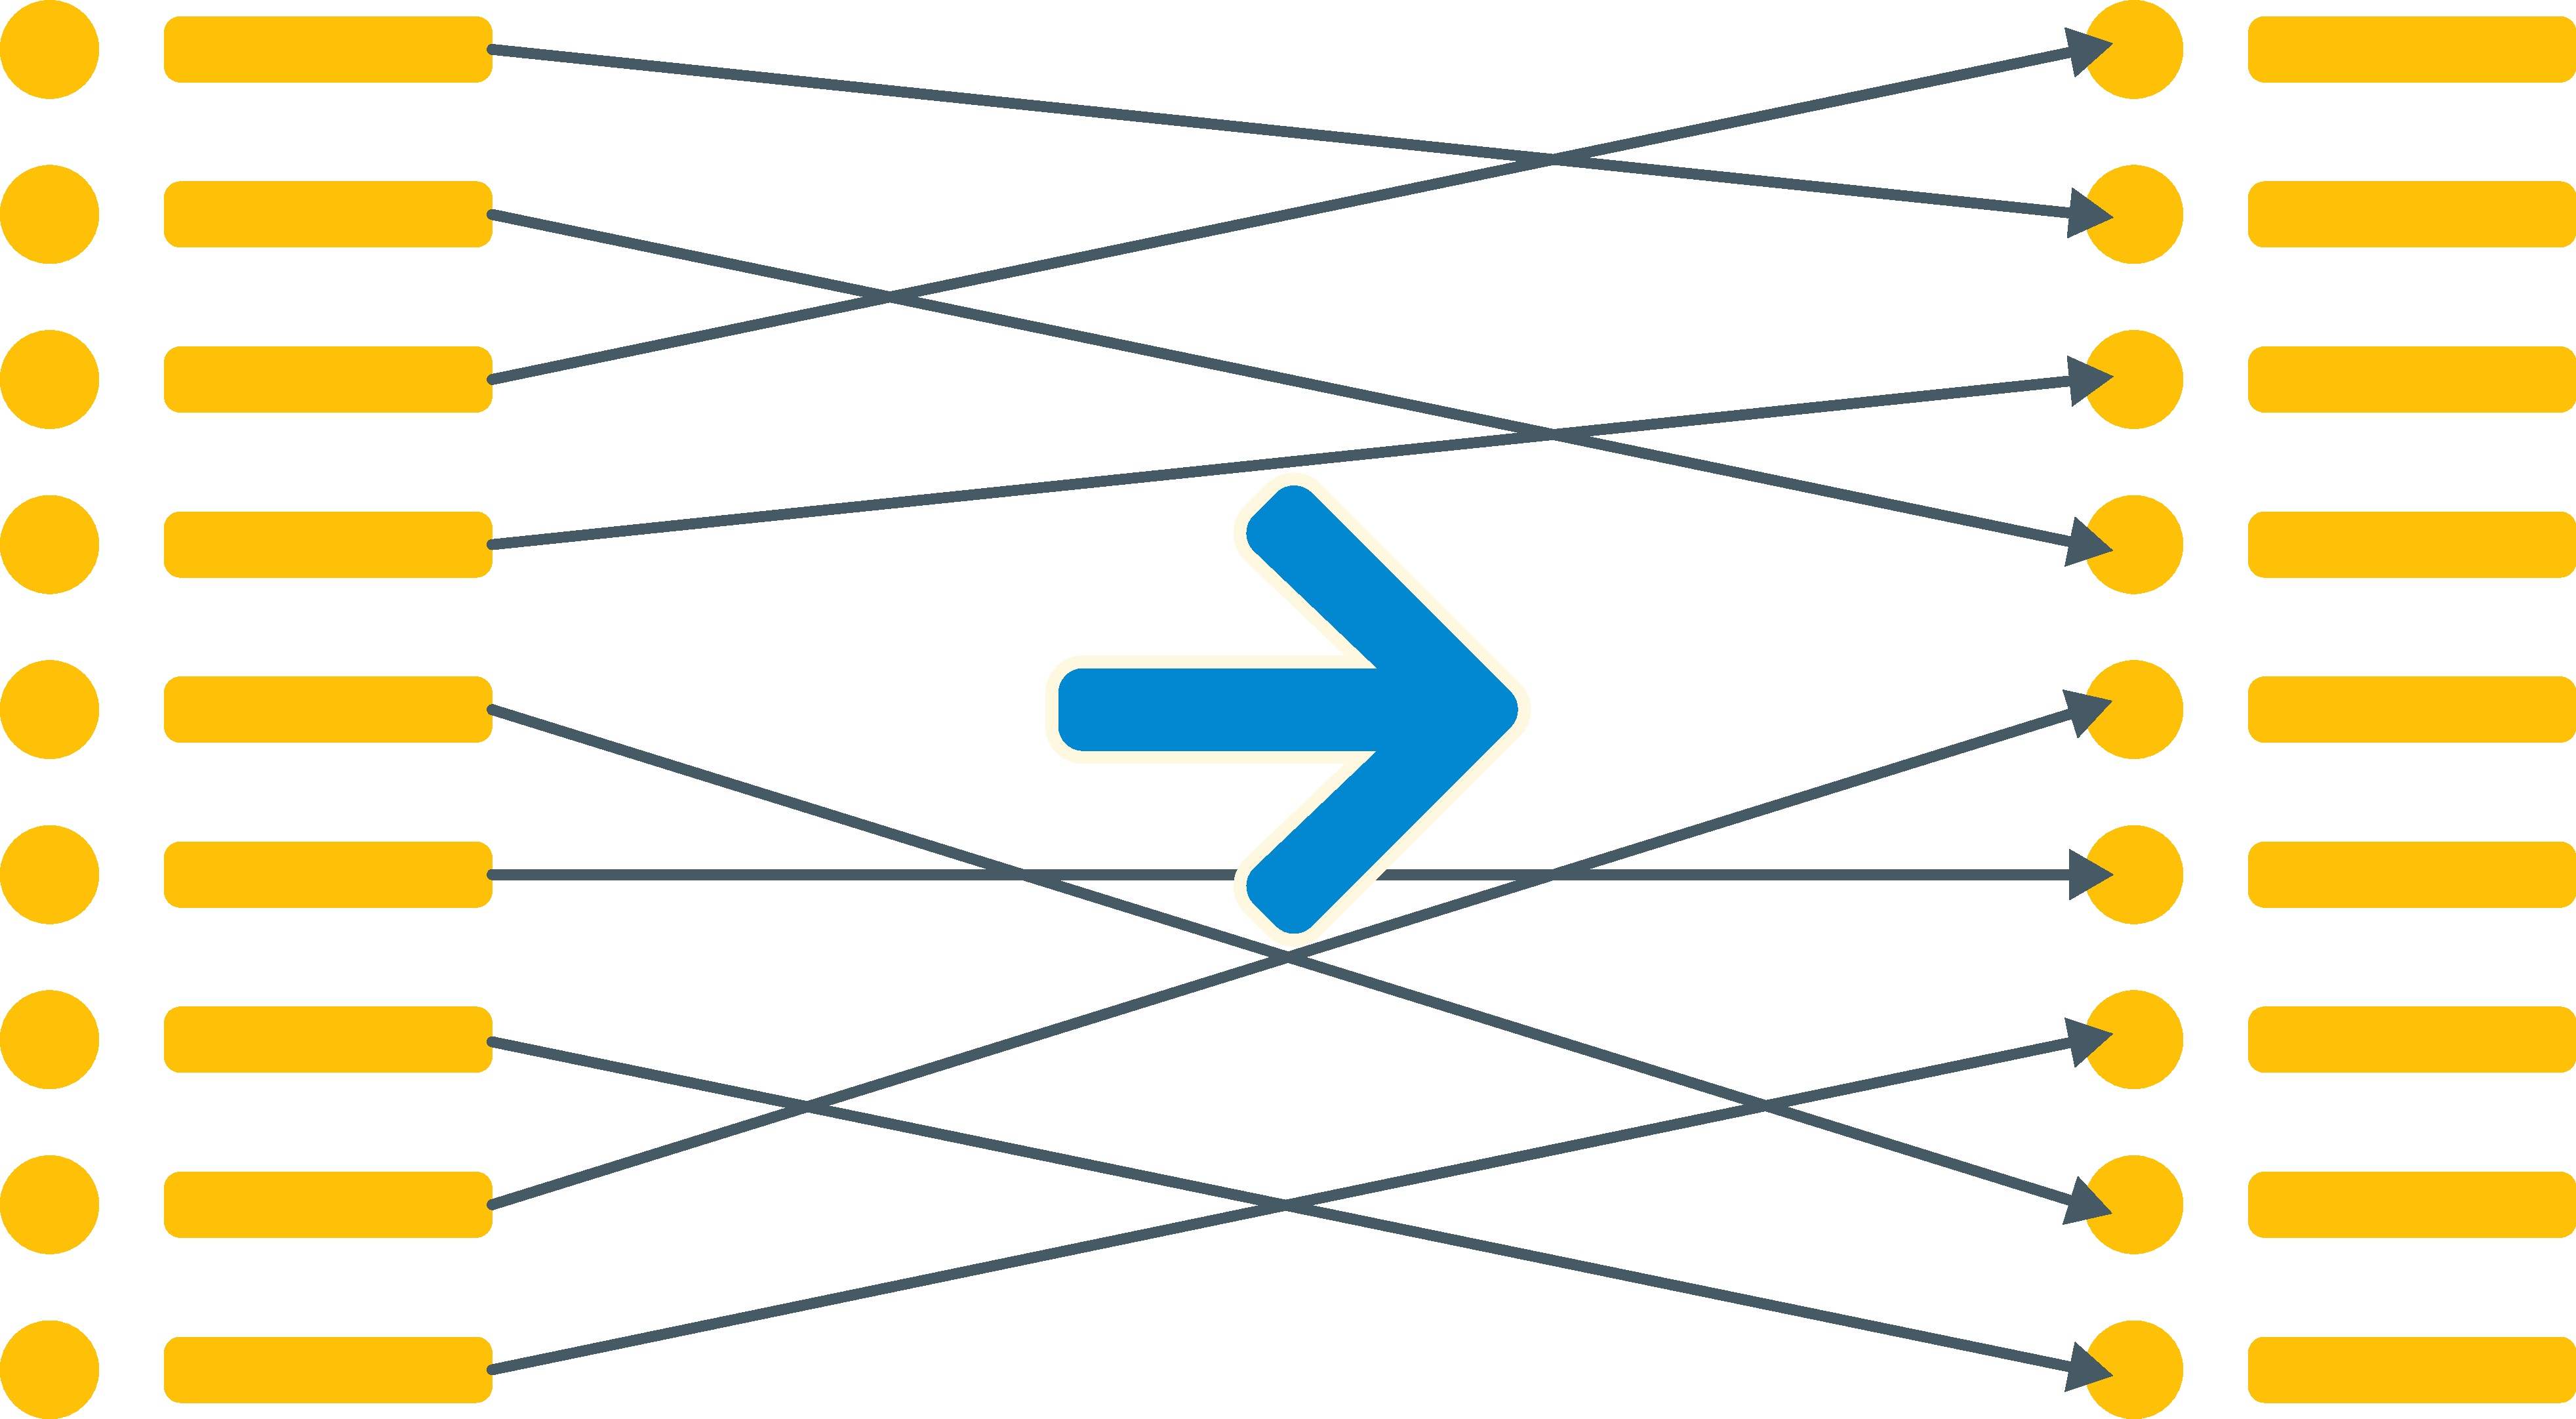
\includegraphics[width=\textwidth]{assets/tikz/approach-tcp.tikz}
	\caption{\tcp{}.}
	\label{fig:tcp}
\end{figure}

\section{Existing implementations}
- OpenClover (enkel Java) heeft hier misschien support voor